\chapter{Kinetic Theory and Particle-in-Cell Simulation}
\label{ch:pic}

The fluid and hybrid treatments developed in preceding chapters close the ion and electron moment equations with assumptions --- a cold or warm mono-energetic ion beam, a Boltzmann electron response, a prescribed collisionality --- that are convenient but not always defensible at the plasma--sheath boundary. The Bohm criterion is, at root, a statement about the low-velocity tail of the ion distribution function, and the ion energy flux $\Gamma_{E}$ this monograph seeks to quantify is an integral over that distribution weighted by kinetic energy. Whenever $f_{\mathrm{i}}(v)$ departs materially from a drifting Maxwellian --- because of a collisionless presheath, a time-varying sheath edge, a non-Maxwellian electron population, or an oblique magnetic field --- a moment-based closure can misrepresent both the total flux and the energy-resolved spectrum a retarding-field or laser diagnostic actually records. This chapter develops the kinetic description of the plasma--wall system from first principles, introduces the particle-in-cell (PIC) method as the primary tool for the self-consistent sheath problem, and explains how PIC-generated data construct synthetic ground truth for validating later inversion algorithms. It closes with the computational cost of kinetic simulation and a survey of reduced kinetic models that make routine sheath-diagnostic work tractable without discarding the physics fluid closures wash out.

\section{The Vlasov and Boltzmann Descriptions}

\subsection{Phase-space distribution functions and the kinetic equation}

The most complete non-relativistic description of a plasma species $s$, short of following every particle trajectory, is the one-particle distribution function $f_{s}(\mathbf{r},\mathbf{v},t)$, defined such that $f_{s}(\mathbf{r},\mathbf{v},t)\,\mathrm{d}^{3}r\,\mathrm{d}^{3}v$ is the expected particle count in the phase-space element at $(\mathbf{r},\mathbf{v})$ at time $t$. All fluid quantities used elsewhere in this monograph are low-order velocity moments of $f_{s}$:
\begin{align}
n_{s}(\mathbf{r},t) &= \int f_{s}(\mathbf{r},\mathbf{v},t)\,\mathrm{d}^{3}v, \\
n_{s}\mathbf{u}_{s}(\mathbf{r},t) &= \int \mathbf{v}\, f_{s}(\mathbf{r},\mathbf{v},t)\,\mathrm{d}^{3}v, \\
p_{s}(\mathbf{r},t) &= \frac{m_{s}}{3}\int |\mathbf{v}-\mathbf{u}_{s}|^{2} f_{s}(\mathbf{r},\mathbf{v},t)\,\mathrm{d}^{3}v = n_{s} T_{s},
\end{align}
with $T_{\mathrm{e}}$ and $T_{\mathrm{i}}$ the electron and ion temperatures used throughout this work. In the absence of collisions, $f_s$ obeys the Vlasov equation, expressing conservation of phase-space density along single-particle trajectories in the self-consistent field:
\begin{equation}
\frac{\partial f_{s}}{\partial t} + \mathbf{v}\cdot\nabla_{\mathbf{r}} f_{s} + \frac{q_{s}}{m_{s}}\left(\mathbf{E} + \mathbf{v}\times\mathbf{B}\right)\cdot\nabla_{\mathbf{v}} f_{s} = 0,
\label{eq:vlasov}
\end{equation}
where $q_{s}$, $m_{s}$ are charge and mass, and $\mathbf{E}$, $\mathbf{B}$ are determined self-consistently from Maxwell's equations (or, in the electrostatic limit relevant to most sheath problems, from Poisson's equation with charge densities given by the zeroth moment of $f_{s}$). Equation~\eqref{eq:vlasov} is linear and hyperbolic; the non-linearity of the plasma problem enters entirely through the coupling of $\mathbf{E}$, $\mathbf{B}$ back to the moments of $f_{s}$ \cite{ref0670}. It is collisionless, an approximation justified whenever the number of particles within a Debye sphere, $N_{\mathrm{D}} = \tfrac{4}{3}\pi n_{\mathrm{e}} \lambda_{\mathrm{D}}^{3}$, is large, so two-body encounters contribute negligibly to the mean-field dynamics.

When binary collisions are not negligible, the right-hand side of Eq.~\eqref{eq:vlasov} acquires a collision operator, yielding the Boltzmann equation,
\begin{equation}
\frac{\partial f_{s}}{\partial t} + \mathbf{v}\cdot\nabla_{\mathbf{r}} f_{s} + \frac{q_{s}}{m_{s}}\left(\mathbf{E} + \mathbf{v}\times\mathbf{B}\right)\cdot\nabla_{\mathbf{v}} f_{s} = \left(\frac{\partial f_{s}}{\partial t}\right)_{\!\mathrm{coll}},
\label{ch13-eq:boltzmann}
\end{equation}
with the collision term written, for elastic binary encounters, in the classical Boltzmann integral form with differential cross-section $\sigma(\mathbf{v},\mathbf{v}';\Omega)$, or, for small-angle Coulomb scattering, in the Fokker--Planck (Landau) form \cite{ref0670}. Both equations are exact conservation statements; the physics of a kinetic model lies entirely in the choice of collision operator, or its omission.

\subsection{Moments, closure, and the failure of fluid models near boundaries}

Multiplying Eq.~\eqref{ch13-eq:boltzmann} by successive powers of $\mathbf{v}$ and integrating generates the familiar hierarchy of fluid moment equations, but each contains a flux term equal to the next-higher moment, so the $n$-th equation always involves an unknown $(n+1)$-th moment. Fluid models close this hierarchy by asserting a relationship between the unclosed moment and lower ones: an equation of state, a Fourier-law heat flux, or, in the cold-ion models used earlier in this monograph, a delta-function or drifting-Maxwellian ion distribution. Such closures are excellent deep in the quasi-neutral bulk, where collisions or turbulent scattering keep $f_{s}$ near local equilibrium.

The closure fails wherever $f_s$ develops structure a low-order moment cannot represent. Three failure modes are of direct relevance to sheath physics:

\begin{enumerate}
\item \textbf{Presheath acceleration without local equilibration.} Ions born at rest are accelerated continuously through the presheath field. If the ion mean free path exceeds the presheath length scale, ions never re-thermalise; the sheath-edge distribution is a strongly non-Maxwellian, one-sided function set by the entire accelerating history, not a local temperature \cite{ref0665,ref0666,ref0659}. This is the regime of the kinetic Tonks--Langmuir model, where the kinetic Bohm criterion --- an inequality on the low-velocity moment of $f_{\mathrm{i}}(v)$, not a fluid drift-speed condition --- must be invoked.
\item \textbf{Trapped and reflected populations.} Electrons (and, in reversing or double-layer sheaths, ions) can be partially reflected, producing a sharp velocity-space cutoff at the local escape energy that a smooth closure cannot represent, but that emerges naturally from the collisionless solution of Eq.~\eqref{eq:vlasov} \cite{ref0670}.
\item \textbf{Non-stationary or oscillating boundaries.} In RF-driven and pulsed sheaths the edge moves on a timescale comparable to, or shorter than, the ion transit time, so the instantaneous distribution superposes sub-populations entering the presheath at different drive phases --- an object no single-temperature closure can capture \cite{ref0637}.
\end{enumerate}

\subsection{When kinetic effects matter: a practical Knudsen-type criterion}

A convenient way to decide whether a fully kinetic treatment is required is to compare the relevant collisional mean free path $\lambda_{\mathrm{mfp}}$ (ion--neutral charge exchange, ion--ion Coulomb scattering, electron--neutral excitation) with the length scale over which the distribution is formed, typically the presheath length $L_{\mathrm{ps}}$:
\begin{equation}
\mathrm{Kn} = \frac{\lambda_{\mathrm{mfp}}}{L_{\mathrm{ps}}}.
\end{equation}
For $\mathrm{Kn} \gg 1$ transport is collisionless and a kinetic treatment is mandatory for energy-resolved quantities such as $\Gamma_{E}$, even though fluid moments like $n_{\mathrm{i}}$ and $u_{\mathrm{i}}$ may remain tolerably accurate. For $\mathrm{Kn}\ll 1$ a corrected fluid closure is usually adequate for the flux itself, though the tail can still deviate since it is populated by the least-collided particles \cite{ref0672}. The intermediate regime $\mathrm{Kn}\sim 1$, common near \SI{1}{\pascal}, is where kinetic simulation is most valuable and analytic theory becomes intractable.

\section{The Particle-in-Cell Method}

\subsection{Superparticles and the discretisation of phase space}

Direct solution of Eq.~\eqref{eq:vlasov} or \eqref{ch13-eq:boltzmann} on a phase-space grid --- the continuum (Eulerian) approach --- is possible, but resolving up to six dimensions is prohibitive for routine scans. PIC instead represents $f_{s}$ as a finite sum of computational \emph{superparticles}, each with a weight $w_{p}$ standing in for many physical particles sharing the same position and velocity:
\begin{equation}
f_{s}(\mathbf{r},\mathbf{v},t) \approx \sum_{p=1}^{N_{p}} w_{p}\, S(\mathbf{r}-\mathbf{r}_{p}(t))\, \delta(\mathbf{v}-\mathbf{v}_{p}(t)),
\end{equation}
where $S$ is a finite-support shape function (commonly linear, ``cloud-in-cell'') that spreads each particle's contribution over neighbouring grid nodes. This converts phase-space transport into the cheaper problem of advancing $N_{p}$ particle-orbit ODEs coupled to a field solve on a spatial grid of far lower dimensionality. Statistical noise from representing smooth $f$ by finite markers scales as $1/\sqrt{N_{p}}$ per cell: more particles reduce noise but raise cost linearly, so particles-per-Debye-length-cell must be chosen with the same care as grid spacing.

\subsection{The PIC cycle: weighting, field solve, force interpolation, particle push}

A single PIC time step advances the system through four operations, per species per step:

\begin{enumerate}
\item \textbf{Charge weighting.} Each superparticle's charge $q_{s}w_{p}$ is deposited onto nearby grid nodes using the shape function $S$ used for force interpolation (avoiding a spurious self-force), giving a grid charge density $\rho(\mathbf{r}_{i})$.
\item \textbf{Field solve.} Poisson's equation (electrostatic PIC, appropriate for most low-temperature sheath problems) or the full Maxwell system is solved on the grid,
\begin{equation}
\nabla^{2}\phi(\mathbf{r}) = -\frac{\rho(\mathbf{r})}{\varepsilon_{0}}, \qquad \mathbf{E}(\mathbf{r}) = -\nabla \phi(\mathbf{r}),
\label{ch13-eq:poisson}
\end{equation}
using a direct or iterative linear solver.
\item \textbf{Force interpolation (gather).} The grid field $\mathbf{E}(\mathbf{r}_{i})$ (and $\mathbf{B}(\mathbf{r}_{i})$ if present) is interpolated back to each particle's position using $S$.
\item \textbf{Particle push.} Position and velocity are advanced by the Lorentz force equation,
\begin{equation}
\frac{\mathrm{d}\mathbf{v}_{p}}{\mathrm{d}t} = \frac{q_{s}}{m_{s}}\left(\mathbf{E}(\mathbf{r}_{p}) + \mathbf{v}_{p}\times\mathbf{B}(\mathbf{r}_{p})\right), \qquad \frac{\mathrm{d}\mathbf{r}_{p}}{\mathrm{d}t} = \mathbf{v}_{p}.
\label{eq:lorentz}
\end{equation}
\end{enumerate}
This weight--solve--gather--push cycle is the discrete analogue of Vlasov--Poisson; its self-consistency --- the field pushing the particles is generated by those particles' own charge density --- makes PIC a genuinely non-linear kinetic solver rather than a test-particle tracer in a fixed field. Foundational applications showed that a fully kinetic, self-consistent simulation reproduces the Bohm-criterion-satisfying presheath and sheath potential profile without any fluid closure \cite{ref0631}, and the method has since been applied to planar, magnetized, and pulsed sheath geometries \cite{ref0633}.

\subsection{Time integration: the Boris algorithm and leapfrog scheme}

The particle push is almost universally integrated using the leapfrog scheme, positions at integer levels $t^{n}$ and velocities at half-integer levels $t^{n+1/2}$:
\begin{align}
\mathbf{r}_{p}^{n+1} &= \mathbf{r}_{p}^{n} + \mathbf{v}_{p}^{n+1/2}\,\Delta t, \\
\mathbf{v}_{p}^{n+1/2} &= \mathbf{v}_{p}^{n-1/2} + \frac{q_{s}\Delta t}{m_{s}}\left(\mathbf{E}_{p}^{n} + \frac{\mathbf{v}_{p}^{n+1/2}+\mathbf{v}_{p}^{n-1/2}}{2}\times\mathbf{B}_{p}^{n}\right).
\end{align}
The magnetic-rotation term, implicit in the velocity average, is solved non-iteratively by the Boris rotation: the electric acceleration is split into two half-steps bracketing an exact, energy-conserving rotation about $\mathbf{B}_{p}^{n}$. The scheme is only second-order accurate but symplectic, introducing no secular energy drift over the $10^{4}$--$10^{6}$ steps typical of a sheath run, which is why it remains standard even in modern implicit and magnetized codes \cite{ref0637}. In magnetized sheaths, where the gyro-period can be the fastest timescale, the push must additionally resolve cyclotron rotation, $\Omega_{c}\Delta t \lesssim 0.2$ ($\Omega_{c}=qB/m$), alongside the electrostatic constraints below \cite{ref0633,ref0637}.

\subsection{Stability and accuracy: CFL, Debye-length resolution, and finite-grid instability}

Explicit electrostatic PIC is subject to three coupled stability requirements that jointly determine $\Delta x$, $\Delta t$, and superparticles per Debye-length cell.

\paragraph{CFL condition.} No particle may cross more than one cell per step:
\begin{equation}
\Delta t \le \frac{\Delta x}{v_{\max}},
\end{equation}
with $v_{\max}$ the fastest particle speed present.

\paragraph{Plasma-period resolution.} The explicit leapfrog scheme is unstable, independent of CFL, if the electron plasma oscillation is not resolved in time:
\begin{equation}
\omega_{\mathrm{pe}}\,\Delta t \lesssim 0.2,
\qquad
\omega_{\mathrm{pe}} = \sqrt{\frac{n_{\mathrm{e}} e^{2}}{\varepsilon_{0} m_{\mathrm{e}}}}.
\label{eq:wpe_dt}
\end{equation}
This is usually the most restrictive condition for dense, low-temperature discharges: a typical run ($n_{\mathrm{e}}\sim\SI{e16}{\per\cubic\metre}$) requires order $10^{5}$--$10^{6}$ steps merely to reach one ion transit time across the presheath.

\paragraph{Debye-length grid resolution and finite-grid instability.} The grid must resolve the electron Debye length,
\begin{equation}
\Delta x \lesssim \lambda_{\mathrm{D}}, \qquad \lambda_{\mathrm{D}} = \sqrt{\frac{\varepsilon_{0} T_{\mathrm{e}}}{n_{\mathrm{e}} e^{2}}},
\end{equation}
with a practical guideline $\Delta x \le (0.5\text{--}1)\,\lambda_{\mathrm{D}}$. If violated, the discrete Poisson solver aliases short-wavelength fluctuations onto long wavelengths, producing a spurious \emph{finite-grid instability} that artificially heats electrons and can distort the presheath structure. Because the sheath is only a few $\lambda_{\mathrm{D}}$ thick, resolving it while also resolving the much larger bulk on a uniform grid can be demanding, motivating non-uniform and curvilinear grids. The particles-per-cell count, $N_{\mathrm{ppc}}$, controls statistical noise in derived quantities such as $\Gamma_{E}$; since relative fluctuation scales as $N_{\mathrm{ppc}}^{-1/2}$, resolving the tail of $f_{\mathrm{i}}(v)$, where $v^{2}$ or $v^{3}$ weighting places most statistical weight, typically needs one to two orders of magnitude more particles per cell than resolving density alone. Table~\ref{tab:pic_stability} summarises these constraints.

\begin{table}[htbp]
\centering
\caption{Principal stability and resolution constraints for explicit electrostatic PIC simulation of a plasma sheath. Quantities are defined in the main text; numerical prefactors are conventional guidelines, not sharp bounds.}
\label{tab:pic_stability}
\begin{tabularx}{\linewidth}{@{}l X l@{}}
\toprule
Constraint & Physical origin & Typical form \\
\midrule
Time-step / plasma period & Explicit leapfrog stability of electron plasma oscillation & $\omega_{\mathrm{pe}}\Delta t \lesssim 0.2$ \\
Time-step / cyclotron period & Accurate resolution of gyromotion in magnetized sheaths & $\Omega_{c}\Delta t \lesssim 0.2$ \\
Time-step / CFL & Particle must not skip a cell per step & $\Delta t \le \Delta x / v_{\max}$ \\
Grid spacing / Debye length & Avoidance of finite-grid (aliasing) heating instability & $\Delta x \lesssim (0.5\text{--}1)\lambda_{\mathrm{D}}$ \\
Particles per cell & Control of statistical noise in $f_{\mathrm{i}}(v)$ and its moments & $N_{\mathrm{ppc}} \gtrsim 10^{2}\text{--}10^{3}$ \\
\bottomrule
\end{tabularx}
\end{table}

\subsection{Boundary conditions at plasma-facing surfaces}

Wall-boundary treatment most distinguishes a sheath-oriented PIC code from a generic bounded-plasma solver. At minimum, an absorbing boundary removes a particle the instant it crosses the wall and deposits its charge there (or in a circuit model, for a floating or capacitively coupled electrode); the accumulated wall charge and bias set the boundary condition for the Poisson solve, Eq.~\eqref{ch13-eq:poisson}. More complete models add secondary electron emission, energy- and angle-dependent reflection, and, for dielectric walls, an accumulating surface-charge density --- effects that alter the sheath potential drop and reflected electron component, and require care to avoid spurious charge non-conservation. This is not a bookkeeping detail: since $\Gamma_{E}$ is evaluated at the wall, any boundary error propagates directly into the synthetic ground-truth spectra used for inversion validation in Section~\ref{sec:synthetic_ground_truth}, and naive treatments introduce spurious low-energy structure in the recorded ion distribution.

\section{Collisions in PIC: Monte Carlo Methods and DSMC Coupling}

\subsection{The null-collision Monte Carlo collision (MCC) algorithm}

Collisions between charged and neutral species are incorporated into an otherwise collisionless PIC push through a Monte Carlo collision (MCC) module, interleaved with the PIC cycle (PIC-MCC). For a uniform, stationary neutral gas of density $n_{\mathrm{n}}$, the probability that a superparticle of speed $v$ undergoes process $k$ (elastic scattering, excitation, ionisation, charge exchange, \ldots) in one step is
\begin{equation}
P_{k}(v) = 1 - \exp\!\big[-n_{\mathrm{n}}\,\sigma_{k}(v)\,v\,\Delta t\big] \approx n_{\mathrm{n}}\,\sigma_{k}(v)\,v\,\Delta t,
\end{equation}
with $\sigma_{k}(v)$ the cross-section. Testing this for every particle and process every step is wasteful; the standard solution is the \emph{null-collision method}, in which a single maximum collision frequency
\begin{equation}
\nu_{\max} = n_{\mathrm{n}}\max_{v}\Big[v\sum_{k}\sigma_{k}(v)\Big]
\end{equation}
sets a fixed total probability $P_{\mathrm{null}}=1-\exp(-\nu_{\max}\Delta t)$; a random subset of particles is selected as candidates, and a second, cross-section-weighted draw decides which process (if any) occurs. This reduces cost from $O(N_{p}\times N_{\mathrm{processes}})$ to $O(N_{p})$ evaluations and is used in essentially all PIC-MCC codes for low-temperature sheath problems \cite{ref0637}. Post-collision velocities are sampled from the relevant cross-section, and ionising collisions create a new electron--ion pair with partitioned energy and momentum.

\subsection{Direct simulation Monte Carlo and its coupling to PIC}

MCC treats the neutral background as a fixed reservoir --- valid when ionisation is low and the gas only weakly heated or depleted. When neutral heating, rarefaction, or strong charge-exchange coupling must be captured self-consistently, the neutral gas is instead represented kinetically via direct simulation Monte Carlo (DSMC): neutral superparticles advance ballistically between cells and undergo binary collisions with a partner drawn stochastically from the same cell, at a rate set by a null-collision scheme. Coupling PIC (charged species) to DSMC (neutrals) lets charge-exchange and elastic ion--neutral collisions modify the neutral distribution self-consistently, which matters where resonant charge exchange dominates ion loss: a fast ion can charge-exchange with a slow neutral, instantly replacing a high-energy trajectory with a near-thermal one and populating a distinct low-energy sub-population in $f_{\mathrm{i}}(v)$ at the sheath edge. Multispecies simulations of the hydrogen plasma sheath, tracking several ionic species and their charge-exchange partners, illustrate the practical importance of resolving this structure kinetically rather than through a single-fluid closure. PIC/test-particle schemes, where a self-consistent PIC-MCC bulk solution provides fields and rates for a separately tracked ensemble of sputtered particles, extend this coupling to transport away from a surface.

\subsection{Coulomb collisions and binary collision models}

Long-range Coulomb interactions are formally already contained in the mean-field Vlasov term insofar as the PIC grid resolves the corresponding wavelengths, but graininess of the finite-$N_{p}$ representation introduces artificial collisionality unless $N_{\mathrm{ppc}}$ is large; capturing the correct small-angle Coulomb scattering rate requires an explicit binary Coulomb-collision (Takizuka--Abe-type) module drawing partners from the same spatial cell. Because Coulomb rates scale steeply with relative velocity ($\propto v^{-3}$), such modules matter for thermalisation of the fast electron tail and for ion--ion collisions reshaping the ion velocity distribution near the sheath edge under instability-enhanced collisionality.

\section{Particle-in-Cell Simulation of Plasma Sheaths}

\subsection{Non-Maxwellian ion and electron tails at the sheath edge}

Kinetic PIC simulation of the collisionless plasma--sheath transition consistently reproduces non-Maxwellian features fluid theory cannot: a low-velocity ion population depleted relative to a Maxwellian (the slowest ions are most efficiently accelerated out of the presheath, a self-selection effect at the heart of the kinetic Bohm criterion \cite{ref0665,ref0666}); a high-velocity tail set by the total presheath potential drop rather than a thermal speed; and a truncated electron distribution from preferential loss of the fastest electrons to the wall, partially compensated by secondary-electron re-emission. Fully kinetic simulations were among the first to demonstrate that the sheath-edge ion distribution satisfies the kinetic Bohm criterion in its integral, not simplified fluid, form, and that the low-velocity tail's shape, not merely its second moment, controls marginal stability \cite{ref0631}. Subsequent studies extended this to magnetized sheaths, where the ion distribution acquires structure from gyromotion projected onto the wall normal and from the Chodura-layer transition preceding the Debye sheath \cite{ref0633,ref0637}.

A further class of non-Maxwellian structure arises from multi-species plasmas. Ion--ion plasma simulations (electronegative discharges, or plasmas with two positive-ion species) show each species developing its own sheath-edge velocity distribution, the lighter species dominating the low-energy portion of the combined flux spectrum and the heavier contributing a sharper peak \cite{ref0655}. Because an inversion algorithm recovering $T_{\mathrm{e}}$, $n_{\mathrm{e}}$, or a sheath-potential waveform implicitly assumes a functional form for $f_{\mathrm{i}}(v)$, quantifying how far a PIC-computed distribution departs from that form is a principal diagnostic use of kinetic simulation.

\subsection{Transient and RF-driven sheath dynamics}

RF and pulsed sources present a qualitatively distinct problem: the sheath edge, and hence the instantaneous accelerating potential, oscillates on a timescale that, for typical drive frequencies (\SIrange{1}{100}{\mega\hertz}), can range from much slower than to faster than the ion transit time. When transit time greatly exceeds the RF period, ions respond only to the time-averaged potential and the energy distribution collapses toward a narrow, quasi-mono-energetic peak; when the two periods are comparable, ions respond to the instantaneous field and the distribution broadens into the bimodal structure long observed in capacitively coupled discharges. PIC is the natural tool for this intermediate regime, tracking each ion's transit history without assuming which limit applies \cite{ref0637}, providing the basis for interpreting retarding-field and mass-spectrometric IEDF measurements \cite{ref0672}.

Two further transients are captured naturally by PIC but essentially inaccessible to a fluid closure. Sheath collapse and reversal --- a rapidly changing bias driving the sheath potential briefly below floating or momentarily positive, permitting a transient electron flux before the sheath re-forms --- requires tracking the full evolving distribution rather than a steady-state moment. The finite relaxation time of the presheath and Chodura-layer structures after a step change in bias or plasma parameters --- the ``formation transient'' --- itself carries diagnostic information about collisionality and ion mass.

\subsection{Synthetic diagnostics extracted from PIC}

A PIC simulation stores, at every step, the full six-dimensional (or reduced 1D3V) phase-space information for every superparticle, making it straightforward to construct \emph{synthetic diagnostics} --- numerically evaluated analogues of a real instrument's response --- essential for closing the loop between kinetic theory and the inversion methodology developed later. Three recur throughout:

\begin{itemize}
\item \textbf{Synthetic retarding-field analyser (RFA) trace.} Ions crossing a virtual detector plane are binned by wall-normal kinetic energy and convolved with the same instrument response function (grid transmission, energy resolution, space-charge-limited transmission) used to interpret an experimental trace.
\item \textbf{Synthetic laser-induced-fluorescence (LIF) spectrum.} A Doppler-resolved velocity-space slice extracted from stored superparticle velocities and convolved with natural and instrumental linewidths, directly comparable with measured ion velocity distributions.
\item \textbf{Synthetic mass-spectrometric IEDF.} Superparticles are additionally binned by mass-to-charge ratio prior to energy binning, reproducing the joint energy--species output of an ion mass spectrometer at the wall.
\end{itemize}
In every case, the synthetic diagnostic is built with the same finite resolution, geometric acceptance, and noise model as the instrument it emulates, so any discrepancy between inversion result and known input is attributable to the inversion algorithm itself, not an unstated diagnostic-model mismatch.

\section{Generating Synthetic Ground Truth for Inversion Validation}
\label{sec:synthetic_ground_truth}

\subsection{The forward--inverse validation loop}

The inversion algorithms developed elsewhere in this monograph take a measured (or synthetic) energy-resolved ion signal and recover underlying plasma parameters --- $T_{\mathrm{e}}$, $n_{\mathrm{e}}$, sheath potential drop, or $\Gamma_{E}$ --- by inverting an assumed forward model. Any such inversion is only as trustworthy as the forward model it inverts, and validating solely against the same simplified analytic model is circular: it tests self-consistency, not physical fidelity. PIC simulation breaks this circularity by supplying a forward model with independent physical content --- the full non-linear Vlasov--Poisson solution, including every non-Maxwellian, transient, and multi-species effect the analytic model simplifies away. The validation loop used here: (i) a PIC simulation runs with fully specified, known input parameters (electron temperature and density, neutral pressure and species, bias waveform, magnetic field, wall properties); (ii) synthetic diagnostic traces are extracted; (iii) only these traces, not the underlying parameters, are passed to the inversion algorithm as if an experimental measurement; and (iv) recovered parameters are compared against the known ground truth, with any discrepancy attributed to inversion error, since generation and recovery are independent stages.

\subsection{Constructing controlled synthetic IEDF datasets}

Building a useful dataset requires a systematic parameter scan exercising the inversion algorithm across its expected operating regimes, deliberately including the non-idealities that motivate a kinetic rather than fluid-forward validation. A representative scan varies independently:
\begin{itemize}
\item electron temperature $T_{\mathrm{e}}$ and density $n_{\mathrm{e}}$, spanning low-temperature processing discharges through space-propulsion plumes;
\item neutral pressure, and hence Knudsen number, from collisionless through collision-dominated;
\item ion species and mass, including multi-species mixtures with distinct charge-exchange partners;
\item bias condition: DC floating and biased walls, single- and dual-frequency RF, and pulsed waveforms;
\item magnetic-field strength and angle, from unmagnetized through strongly magnetized, oblique-field Chodura-layer conditions.
\end{itemize}
For each combination, the PIC-computed sheath-edge ion energy distribution and resulting energy flux,
\begin{equation}
\Gamma_{E} = \int_{0}^{\infty} \tfrac{1}{2} m_{\mathrm{i}} v^{2}\; v\, f_{\mathrm{i}}(v)\,\mathrm{d}v,
\end{equation}
serve as the exact ground truth against which any reduced-model or inverted estimate of $\Gamma_{E}$ is scored. Because $\Gamma_{E}$ is weighted by $v^{3}$, it is disproportionately sensitive to the correctly resolved high-velocity tail --- exactly the feature a coarse fluid model is most likely to misrepresent. Figure~\ref{fig:iedf_schematic} sketches the qualitative distinction between a drifting-Maxwellian distribution assumed by a simple analytic forward model and the broadened, high-energy-skewed distribution characteristic of a kinetically resolved collisionless presheath.

\begin{figure}[htbp]
\centering
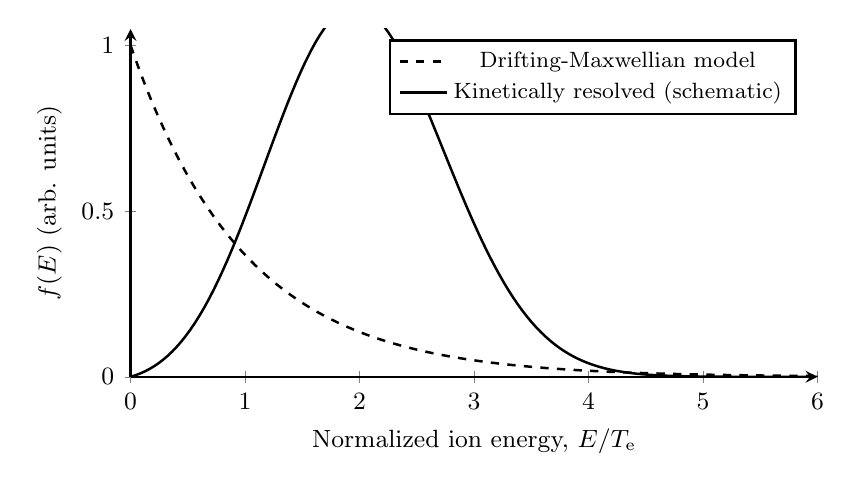
\begin{tikzpicture}
\begin{axis}[
 width=0.85\linewidth,
 height=6cm,
 xlabel={Normalized ion energy, $E/T_{\mathrm{e}}$},
 ylabel={$f(E)$ (arb. units)},
 xmin=0, xmax=6,
 ymin=0, ymax=1.05,
 axis lines=left,
 grid=none,
 legend pos=north east,
 ticklabel style={font=\small},
 label style={font=\small},
 legend style={font=\footnotesize, draw=black},
 line width=0.9pt,
]
\addplot[domain=0:6, samples=100, black, dashed] {exp(-x)};
\addlegendentry{Drifting-Maxwellian model}
\addplot[domain=0:6, samples=150, black, solid] {(x/1.6)*exp(-(x-1.6)^2/1.4)};
\addlegendentry{Kinetically resolved (schematic)}
\end{axis}
\end{tikzpicture}
\caption{Schematic comparison of two normalized ion energy distributions at the sheath edge: a single-exponential form implied by a drifting-Maxwellian analytic forward model (dashed), and a qualitatively broadened, peaked profile representative of a kinetically resolved collisionless-presheath calculation (solid). Both curves are illustrative analytic functions; neither represents measured or simulated data.}
\label{fig:iedf_schematic}
\end{figure}

\subsection{Noise injection, forward diagnostic models, and blind validation}

A dataset too clean --- free of the counting statistics, finite resolution, and systematic offsets present in any real instrument --- risks validating the inversion algorithm only in an unrealistically favourable regime. The synthetic traces are therefore processed through an explicit forward instrument model: Poisson counting noise set by an assumed integration time and detector sensitivity; a finite energy-resolution kernel (typically Gaussian, width set by grid transmission and analyser geometry) convolved with the ideal spectrum; and, where relevant, a slowly varying baseline representing secondary-electron background. Because the entire chain from PIC parameters through extraction, noise injection, and inversion is under the analyst's control, a strict \emph{blind} validation is possible, in which generating parameters are withheld from whoever runs the inversion until after the result is reported.

\section{Computational Cost and Reduced Models}

\subsection{Scaling of PIC cost with dimensionality and disparate scales}

The cost of an explicit electrostatic PIC simulation scales, at fixed domain size and duration, as the product of grid cells, superparticles per cell, and time steps. Each factor is set by a physical scale-separation ratio that is generically large in a real plasma--sheath system:
\begin{itemize}
\item cells spanning a domain of size $L$ while resolving $\lambda_{\mathrm{D}}$ scale as $(L/\lambda_{\mathrm{D}})^{d}$ in $d$ dimensions;
\item time steps needed to reach duration $\tau$ while resolving $\omega_{\mathrm{pe}}^{-1}$ (Eq.~\eqref{eq:wpe_dt}) scale as $\tau\,\omega_{\mathrm{pe}}$;
\item the mass ratio $m_{\mathrm{i}}/m_{\mathrm{e}}$ ($\sim 1.8\times10^{3}$ for hydrogen, up to $2\text{--}5\times10^{5}$ for heavy propellants) sets how many electron plasma periods must be resolved before the much slower ion transit, on which the sheath and presheath reach quasi-steady state, can be observed.
\end{itemize}
Because sheath-diagnostic applications span from a sub-millimetre sheath to a centimetre-to-metre bulk region, and ion transit time can exceed the electron plasma period by five or six orders of magnitude, a fully resolved, explicit electrostatic PIC simulation of an entire discharge is expensive even on HPC hardware, and a fully 3D, electromagnetic, multi-species run can require weeks of computation per operating point. This motivates the hierarchy of reduced and hybrid kinetic models below, each trading fidelity for cost, each validated against the fully kinetic ground truth of Section~\ref{sec:synthetic_ground_truth}.

\subsection{Hybrid and reduced-order kinetic models}

The most widely used cost-reduction strategy is the \emph{hybrid} approach: the computationally cheap species (usually electrons, whose small mass drives the restrictive $\omega_{\mathrm{pe}}\Delta t$ constraint) is treated with a fast fluid or Boltzmann-relation closure, while the species carrying the diagnostic information (usually ions) remains kinetic. Removing the electron plasma-period constraint lets the time step be set by the slower ion dynamics, typically a speed-up of two to three orders of magnitude. Hybrid fluid-electron/kinetic-ion schemes are the standard tool for large-scale Hall-thruster discharge modelling, where benchmarking against kinetic and experimental data shows where the hybrid closure remains valid and where it misses electron-kinetic effects such as anomalous cross-field transport \cite{ref0433}.

\subsection{Semi-kinetic trajectory simulation}

A further cost reduction, specific to the magnetized sheath and presheath problem, is \emph{kinetic trajectory simulation}: rather than a large ensemble of freely evolving superparticles subject to a mean field recomputed every step, a small number of representative ion trajectories are integrated through an iteratively determined potential profile, itself updated by enforcing quasi-neutrality using the trajectory-ensemble moments. Because the potential update, not an explicit field solve every step, is rate-limiting, this achieves substantial cost reduction while retaining the essential kinetic feature: an ion distribution built up self-consistently from particle histories rather than assumed \emph{a priori}. It has been developed for the 1D3V magnetized sheath, resolving the coupled presheath--Chodura-layer--Debye-sheath structure, and extended to multi-component sheaths tracking several ion species. Replacing the noisy explicit field solve with a smoother iterative construction yields low-noise distributions at a fraction of the cost, at the price of restricted geometry and a modeller-supplied coupling ansatz.

\subsection{Continuum kinetic (Vlasov) solvers as an alternative to particle noise}

A conceptually distinct route replaces the particle (Lagrangian, Monte-Carlo-sampled) representation of $f_{s}$ with a direct, grid-based (Eulerian) discretisation of the Vlasov equation, using finite-volume, spectral, or discontinuous-Galerkin methods on a phase-space mesh. Such solvers rely on no random sample and are entirely free of the statistical noise limiting the resolvable tail of $f_{\mathrm{i}}(v)$ in a standard PIC run, at the cost of a higher-dimensional grid and steeper memory/arithmetic scaling. Continuum kinetic and multi-fluid comparisons of classical sheath structure have quantified when a fluid closure remains adequate and when the noise-free continuum solution reveals structure a comparable-cost particle simulation would not resolve above its own statistical floor \cite{ref0659}. Reduced-basis and moment-closure techniques applied to the Vlasov system offer a further avenue for cost reduction. Because $\Gamma_{E}$ is a high-order moment disproportionately sensitive to the well-resolved tail, this monograph's ground-truth campaign favours high-$N_{\mathrm{ppc}}$ PIC runs, cross-checked where affordable against continuum benchmarks.

\section{Summary}

This chapter developed the kinetic foundation on which the synthetic ground-truth generation used elsewhere in this monograph rests. The Vlasov and Boltzmann equations were introduced as the exact phase-space description from which all fluid closures are derived by truncated moment-taking, and the circumstances under which that truncation fails at a plasma boundary --- collisionless presheath acceleration, trapped and reflected populations, non-stationary sheath edges --- were connected to the non-Maxwellian structure of $f_{\mathrm{i}}(v)$ that a kinetic Bohm criterion, rather than its fluid form, correctly captures. The particle-in-cell method was presented as the standard tool for solving Vlasov--Poisson in this regime, with attention to the weight--solve--gather--push cycle, the Boris integration scheme, and the coupled CFL, plasma-period, and Debye-length constraints that determine the grid, time step, and particle count a credible simulation must use. Monte Carlo collision and DSMC-coupled schemes extend this framework to collisional and multi-species regimes, and a survey of PIC studies of non-Maxwellian sheath structure, transient and RF-driven dynamics, and synthetic diagnostic extraction established the phenomena --- depleted low-velocity ion tails, RF-broadened bimodal distributions, multi-species flux partitioning --- that make a fully kinetic forward model indispensable for inversion validation. The chapter's central contribution is the forward--inverse validation loop of Section~\ref{sec:synthetic_ground_truth}, in which PIC-generated, noise-injected synthetic traces provide an independent ground truth for blind-testing later inversion algorithms. Finally, because PIC cost scales unfavourably with the disparate length and time scales of the plasma--sheath system, the chapter surveyed hybrid, semi-kinetic trajectory, and continuum alternatives that make routine, parameter-scanned kinetic sheath analysis practical, noting that the high-order moment defining $\Gamma_{E}$ places disproportionate demands on tail resolution that only a well-resolved kinetic calculation can reliably supply.
